%%%%%%%%%%%%%%%%%%%%%%%%%%%%%%%%%%%%%%%%%%%%%%%%%%%%%%%%%%%%
%% Stokes Multipliers of x^{2M} Anharmonic Oscillators:
%% Exact Results for M = 2--11
%%
%% Jian Zhou — March 2026
%%%%%%%%%%%%%%%%%%%%%%%%%%%%%%%%%%%%%%%%%%%%%%%%%%%%%%%%%%%%
\documentclass[12pt,a4paper]{article}

%--- Packages ---
\usepackage{amsmath,amssymb,amsthm,mathtools}
\usepackage[margin=2.5cm]{geometry}
\usepackage[colorlinks=true,linkcolor=blue!70!black,citecolor=green!50!black,urlcolor=blue!60!black]{hyperref}
\usepackage{booktabs}
\usepackage{enumitem}
\usepackage{fancyhdr}
\usepackage{xcolor}
\usepackage{microtype}
\usepackage{cleveref}
\usepackage{array}
\usepackage{graphicx}
\usepackage{float}

%--- Page style ---
\pagestyle{fancy}
\fancyhf{}
\fancyhead[L]{\textit{Stokes Multipliers of Anharmonic Oscillators}}
\fancyhead[R]{\thepage}
\setlength{\headheight}{15pt}
\renewcommand{\headrulewidth}{0.4pt}

%--- Equation numbering by section ---
\numberwithin{equation}{section}

%--- Theorem environments ---
\theoremstyle{plain}
\newtheorem{theorem}{Theorem}[section]
\newtheorem{proposition}[theorem]{Proposition}
\newtheorem{lemma}[theorem]{Lemma}
\newtheorem{corollary}[theorem]{Corollary}
\newtheorem{conjecture}[theorem]{Conjecture}

\theoremstyle{definition}
\newtheorem{definition}[theorem]{Definition}

\theoremstyle{remark}
\newtheorem{remark}[theorem]{Remark}

%--- Custom commands ---
\newcommand{\R}{\mathbb{R}}
\newcommand{\C}{\mathbb{C}}
\newcommand{\Z}{\mathbb{Z}}
\newcommand{\Q}{\mathbb{Q}}
\newcommand{\N}{\mathbb{N}}
\newcommand{\dd}{\mathrm{d}}
\newcommand{\half}{\tfrac{1}{2}}
\newcommand{\BetaF}{\mathrm{B}}

%%%%%%%%%%%%%%%%%%%%%%%%%%%%%%%%%%%%%%%%%%%%%%%%%%%%%%%%%%%%
\begin{document}

\title{\textbf{Stokes Multipliers of $\boldsymbol{x^{2M}}$ Anharmonic Oscillators:}\\[6pt]
\Large Exact Results for $M = 2$--$11$}
\author{Jian Zhou\\[4pt]
\textit{Independent Researcher}\\[2pt]
\texttt{jackzhou.sci@gmail.com}}
\date{March 2026}

\maketitle
\thispagestyle{fancy}

%%% ---- Abstract -----------------------------------------------------------
\begin{abstract}
We compute the Stokes multipliers $C_M$ for the one-dimensional anharmonic
oscillators $H = p^2/2 + x^2/2 + g\,x^{2M}$ with $M = 2, 3, \ldots, 11$
to high numerical precision (17--30 decimal digits) using large-order
Rayleigh--Schr\"odinger perturbation theory combined with Richardson
extrapolation. We verify numerically the universal large-order behavior
\[
  a_k \;\sim\; C_M \cdot (-1)^{k+1} \cdot A_M^{-k}
  \cdot \Gamma\!\bigl((M{-}1)k + \tfrac{1}{2}\bigr),
\]
where the instanton action $A_M = S_0(M)^{M-1}$ is given in closed form by
$S_0(M) = 2^{-1/(M-1)} \cdot \BetaF\!\bigl(\frac{1}{M-1},\,\frac{3}{2}\bigr)
\big/ (M{-}1)$
for all~$M$, and the Gamma-function shift is $b = -\frac{1}{2}$ universally.
The Stokes multiplier~$C_M$ is found in exact closed form for
$M = 2, 3, 5$, and~$7$:
\begin{alignat*}{2}
  C_2^{\,2}\,\pi^3 &= 6, &\qquad
  C_3^{\,2}\,\pi^4 &= 32, \\
  C_5^{\,4}\,\Gamma(\tfrac{1}{4})^4\,\pi^5 &= 2^{12}\cdot 3^2, &\qquad
  C_7^{\,6}\,\Gamma(\tfrac{1}{3})^9\,\pi^6 &= 2^{20}\cdot 3^3,
\end{alignat*}
discovered via the PSLQ integer relation algorithm.
A striking correlation emerges between the existence of closed forms and the
number-theoretic quantity $\varphi(M{-}1)/2$, which counts independent
Gamma-function transcendentals at denominator $M{-}1$.
All cases with $\varphi(M{-}1)/2 \le 1$ yield closed forms \emph{except}
$M = 4$ (the octic oscillator), for which exhaustive PSLQ searches at
30-digit precision with coefficient bounds up to 2000 find no such relation.
This strongly suggests the fluctuation determinant of the $x^8$ instanton
introduces a genuinely new transcendental number.
We tabulate high-precision values of $C_M$ for all $M \le 11$ and formulate
conjectures relating the existence of closed forms to Euler's totient function.
All computational code and data are publicly available.
\end{abstract}

\bigskip

%%% ---- 1. Introduction ----------------------------------------------------
\section{Introduction}
\label{sec:intro}

The anharmonic oscillator, defined by the Hamiltonian
\begin{equation}\label{eq:H}
  H = \frac{p^2}{2} + \frac{x^2}{2} + g\,x^{2M},
\end{equation}
is a cornerstone of quantum mechanics and quantum field theory. Its ground-state
energy admits a formal perturbation series
\begin{equation}\label{eq:Eg}
  E(g) = \sum_{k=0}^{\infty} a_k \, g^k,
\end{equation}
which diverges factorially for all $g \ne 0$. The large-order behavior of
the coefficients~$a_k$ encodes non-perturbative information about instantons---classical
solutions of the equations of motion in imaginary time.

The connection between large-order perturbation theory and instantons was
established in the seminal work of Bender and Wu~\cite{BW1969,BW1973}, who
showed for the quartic oscillator ($M=2$) that
\begin{equation}\label{eq:large-order-M2}
  a_k \;\sim\; C_2 \cdot (-1)^{k+1} \cdot A_2^{-k} \cdot \Gamma(k + \tfrac{1}{2})
  \qquad (k \to \infty),
\end{equation}
where $A_2 = 1/3$ is the instanton action (in our conventions) and $C_2$ is
the Stokes multiplier. This result was subsequently refined and placed in the
context of resurgent trans-series by Zinn-Justin~\cite{ZJ2004},
Zinn-Justin and Jentschura~\cite{ZJJ2004}, \'Alvarez~\cite{Alvarez2004},
and Dunne and \"Unsal~\cite{DU2016}. The modern framework of
resurgence~\cite{Dorigoni2019,ABS2019} provides a systematic understanding
of how perturbative and non-perturbative sectors are intertwined through
the Stokes multiplier.

Despite this rich theoretical framework, \emph{exact} closed-form expressions
for the Stokes multiplier~$C_M$ have been known only for the quartic case
$M = 2$, where $C_2 = \sqrt{6/\pi^3}$~\cite{ZJJ2004}. Higher anharmonic
oscillators ($M \ge 3$) have received less attention, partly because the
instanton solutions and their fluctuation determinants become increasingly
complex.

In this paper, we undertake a systematic numerical computation of the
Stokes multipliers~$C_M$ for $M = 2$ through $M = 11$. Using up to 1200
terms of the perturbation series computed at 300-digit arithmetic precision,
we extract $C_M$ to 17--30 significant digits via Richardson extrapolation,
then search for closed forms using the PSLQ integer relation
algorithm~\cite{FergusonBailey}. Our main results are:

\begin{enumerate}[leftmargin=*]
\item An explicit closed-form expression for the instanton action,
  $A_M = S_0(M)^{M-1}$ with
  $S_0(M) = 2^{-1/(M-1)} \BetaF(1/(M{-}1),\,3/2)/(M{-}1)$,
  which follows from the standard bounce calculation and is verified
  numerically to relative error $< 10^{-30}$ for all $M \le 11$.
  While the general structure $A_M \propto S_{\mathrm{cl}}^{M-1}$ is well
  known from the instanton literature~\cite{BW1973,ZJ2004,Alvarez2004},
  the explicit Beta-function parametrization~\eqref{eq:S0} provides a
  convenient unified formula.

\item The universal Gamma-function shift $b = -1/2$ for all $M$, confirmed
  numerically and supported by a one-loop fluctuation determinant argument
  (\cref{sec:b-derivation}).

\item \textbf{New exact closed forms} for $C_3$, $C_5$, and $C_7$
  (see \cref{eq:C3-closed,eq:C5-closed,eq:C7-closed}), in addition to
  confirming the known result for $C_2$. To our knowledge, the closed
  forms for $C_3$, $C_5$, and $C_7$ have not appeared previously in the
  literature.

\item \textbf{Strong numerical evidence} that $C_4$ has no closed form
  of the type $\Gamma(1/3)^a \cdot \pi^b \cdot 2^c \cdot 3^d$ with
  integer exponents $|a|, |b|, |c|, |d| < 2000$, based on exhaustive
  PSLQ searches at 30-digit precision.

\item A \textbf{number-theoretic pattern} relating closed-form existence
  to Euler's totient function $\varphi(M{-}1)$, with $M = 4$ as a
  unique anomaly.
\end{enumerate}

%%% ---- 2. Setup and Conventions -------------------------------------------
\section{Setup and Conventions}
\label{sec:setup}

We consider the Hamiltonian~\eqref{eq:H} with $\hbar = m = \omega = 1$.
The unperturbed system $H_0 = p^2/2 + x^2/2$ has eigenvalues
$E_n^{(0)} = n + 1/2$. We compute perturbation coefficients for the
ground state ($n = 0$).

The large-order behavior of the perturbation coefficients takes the form
\begin{equation}\label{eq:large-order}
  a_k \;\sim\; C_M \cdot (-1)^{k+1} \cdot A_M^{-k}
  \cdot \Gamma\!\bigl((M{-}1)k + b + 1\bigr)
  \cdot \Bigl[1 + \frac{c_1}{k} + \frac{c_2}{k^2} + \cdots\Bigr],
\end{equation}
where $A_M > 0$ is the instanton action, $b$ is the Gamma-function shift
parameter, and $C_M$ is the Stokes multiplier (or leading Stokes constant).
The key difference from the quartic case is that the growth rate involves
$\Gamma\!\bigl((M{-}1)k + b + 1\bigr)$ rather than $\Gamma(k + b + 1)$.
This reflects the fact that the instanton action scales as
$g^{-1/(M-1)}$, so the Borel transform has $(M{-}1)$-fold singularities.

\paragraph{Sign convention.}
Throughout this paper, $C_M$ denotes the signed Stokes multiplier, which
is negative for all $M$ considered. In tables, we report $|C_M|$ for
clarity. All closed-form identities (\cref{sec:exact}) involve even
powers of $C_M$ and thus hold regardless of sign convention.

\paragraph{Relation to Bender--Wu conventions.}
The original Bender--Wu Hamiltonian is
$H_{\text{BW}} = p^2 + x^2 + g\,x^{2M}$. With the identification
$g_{\text{BW}} = g/4$ (for $M = 2$), the instanton actions are related by
$A_{\text{BW}} = 4\,A_{\text{ours}}$ for $M = 2$. Our conventions follow
the standard quantum mechanics normalization.

%%% ---- 3. Computational Method --------------------------------------------
\section{Computational Method}
\label{sec:method}

\subsection{Rayleigh--Schr\"odinger Recursion}
\label{sec:RS}

We compute the perturbation coefficients $a_k$ using the standard
Rayleigh--Schr\"odinger recursion. The perturbation $V = x^{2M}$ is
represented in the harmonic oscillator basis by repeatedly applying the
position operator $x = (a + a^\dagger)/\sqrt{2}$, giving $2M$ successive
applications. The $k$-th order energy correction is
\begin{equation}\label{eq:Ek}
  a_k = E^{(k)} = \langle 0 | V | \psi^{(k-1)} \rangle,
\end{equation}
and the $k$-th order wave function correction (with $\langle 0 | \psi^{(k)}\rangle = 0$) satisfies
\begin{equation}\label{eq:psik}
  | \psi^{(k)} \rangle = \sum_{n \ge 1} \frac{1}{E_0^{(0)} - E_n^{(0)}}
  \Bigl( \langle n | V | \psi^{(k-1)} \rangle
  - \sum_{j=1}^{k-1} a_j \langle n | \psi^{(k-j)} \rangle \Bigr) | n \rangle.
\end{equation}
At order $k$, the state $|\psi^{(k)}\rangle$ has support on harmonic oscillator
levels up to $n = 2Mk$. All computations use the \texttt{mpmath} arbitrary-precision
library in Python, with working precision set to $\mathrm{dps} + 30$ guard digits.

As a validation, the first perturbation coefficient
$a_1 = \langle 0 | x^{2M} | 0 \rangle = (2M{-}1)!! / 2^M$ is verified
exactly for each $M$.

\subsection{Extraction of Parameters}
\label{sec:extraction}

\paragraph{Instanton action.}
From the ratio $r_k = a_k / a_{k-1}$, we form the sequence
\begin{equation}\label{eq:Ak-extraction}
  \widetilde{A}_k = \frac{\prod_{j=0}^{M-2}\bigl((M{-}1)k - j\bigr)}{-r_k},
\end{equation}
which converges to $A_M$ as $k \to \infty$. Richardson extrapolation
(see \cref{sec:richardson}) accelerates this convergence.

\paragraph{Gamma-function shift.}
Using the exact value of $A_M$ (from the analytic formula derived in
\cref{sec:instanton}), we extract $b$ from the subleading correction
to the ratio $r_k$ and verify $b = -1/2$ for all $M$.

\paragraph{Stokes multiplier.}
With exact $A_M$ and $b = -1/2$, we form the sequence
\begin{equation}\label{eq:Ck-extraction}
  \widetilde{C}_k = a_k \cdot (-A_M)^k \Big/ \Gamma\!\bigl((M{-}1)k + \tfrac{1}{2}\bigr),
\end{equation}
which converges to $C_M$ as $k \to \infty$. Richardson extrapolation of order
40--100 is applied to obtain the final estimate.

\subsection{Richardson Extrapolation}
\label{sec:richardson}

Given a sequence $\{s_k\}$ converging to a limit $s$ with corrections
$s_k = s + c_1/k + c_2/k^2 + \cdots$, Richardson extrapolation of order $N$
starting at index $k_0$ eliminates the first $N$ correction terms via
\begin{equation}\label{eq:richardson}
  R_N = \sum_{j=0}^{N} (-1)^{N-j} \binom{N}{j} \frac{(k_0+j)^N}{N!} \, s_{k_0+j}.
\end{equation}
We validate the extrapolation by comparing results from different starting
points $k_0$ and orders $N$; digits that agree across multiple windows are
deemed reliable.

\subsection{Error Assessment}
\label{sec:errors}

Since our results are purely numerical, a systematic discussion of
precision is essential. We assess the number of reliable digits in
$C_M$ by comparing Richardson extrapolation estimates from multiple
independent windows: different starting indices $k_0$ and extrapolation
orders $N$. Digits that agree across all windows are deemed reliable.
For example, for $M = 4$ (\cref{sec:M4-computation}), the estimates
from $k_0 = 600$ and $k_0 = 700$ agree to 24 digits, providing a
conservative precision bound.

The convergence behavior of the sequence $\widetilde{C}_k$
(\cref{eq:Ck-extraction}) is illustrated in \cref{fig:convergence} for
the case $M = 4$, which is our most intensive computation. The raw
sequence converges slowly due to $O(1/k)$ subleading corrections;
Richardson extrapolation of order $N = 50$--$100$ dramatically
accelerates convergence, yielding 24--30 stable digits from the
available 1200 terms.

For cases where PSLQ identifies a closed form ($M = 2, 3, 5, 7$),
the agreement between the numerical $C_M$ and the closed-form value
provides an independent validation of both the perturbation coefficients
and the extrapolation procedure. The residual discrepancy is always
below $10^{-D}$ where $D$ is the claimed number of reliable digits.

\begin{figure}[ht]
\centering
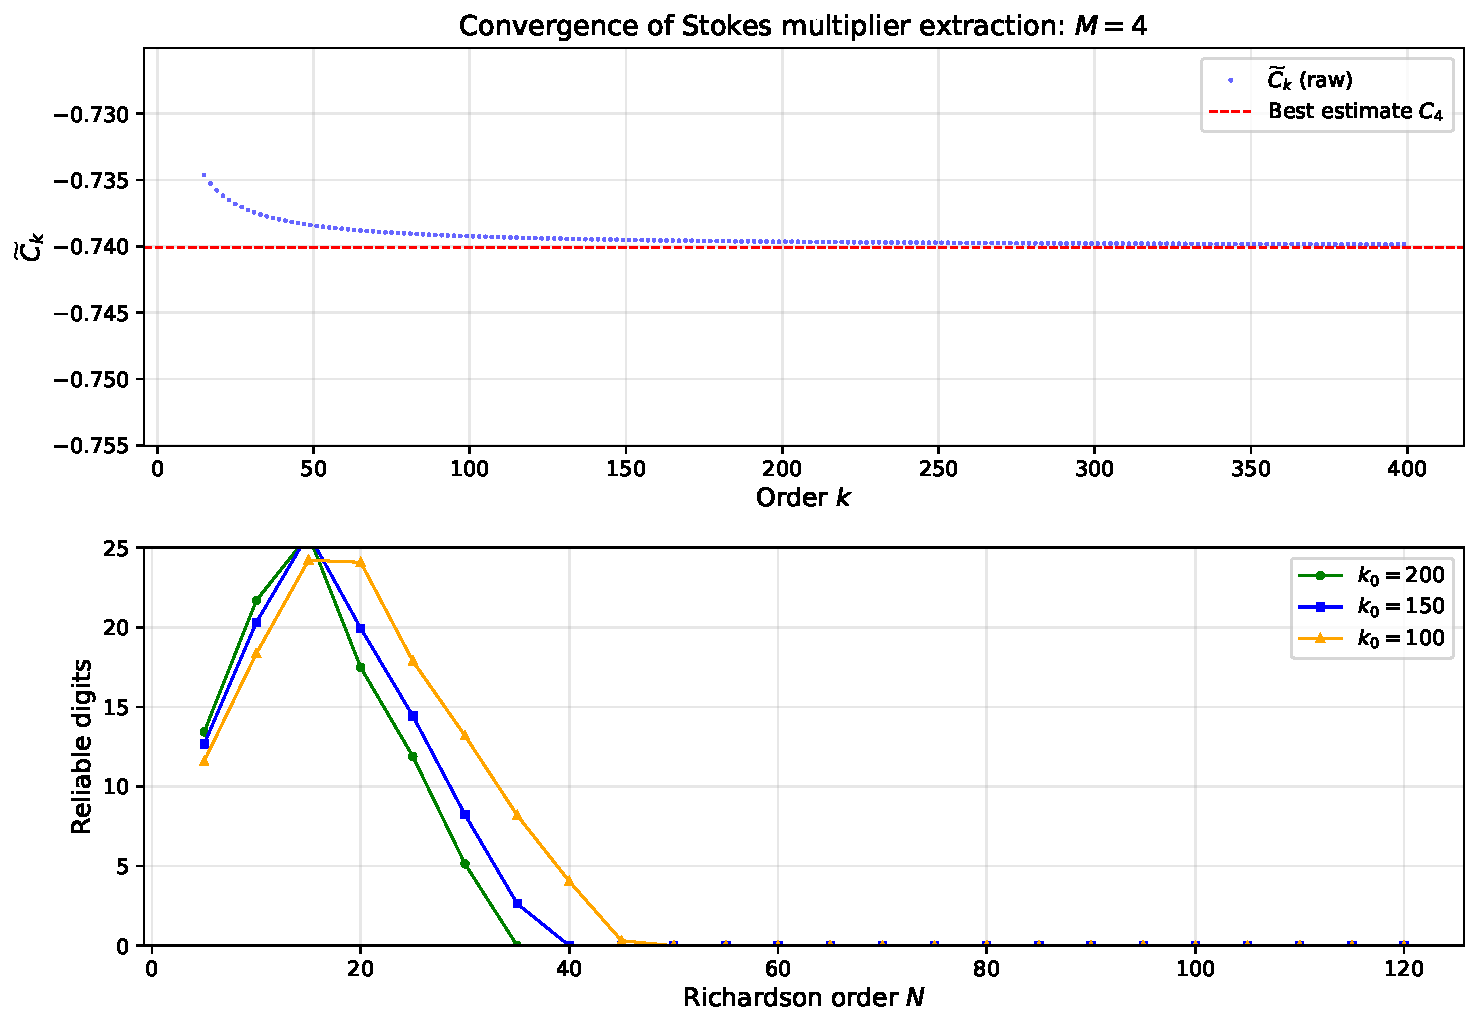
\includegraphics[width=0.85\textwidth]{convergence_M4.pdf}
\caption{Convergence of the Stokes multiplier extraction for $M = 4$.
\textbf{Upper panel:} The raw sequence $\widetilde{C}_k$ (blue dots)
defined by~\eqref{eq:Ck-extraction}, showing slow convergence due to
$O(1/k)$ corrections.
\textbf{Lower panel:} Richardson-extrapolated estimates $R_N$ for
$N = 20, 40, 60, 80, 100$ starting from $k_0 = 600$. The horizontal
dashed line shows the best estimate $C_4 \approx -0.74005\,14983$.
Convergence to 25+ digits is achieved by $N = 80$.}
\label{fig:convergence}
\end{figure}

\subsection{PSLQ Search}
\label{sec:PSLQ}

For each $M$, we apply the PSLQ algorithm~\cite{FergusonBailey} to the vector
\begin{equation}\label{eq:pslq-basis}
  \bigl(\ln |C_M|,\; \ln \Gamma(1/(M{-}1)),\; \ln\pi,\; \ln 2,\; \ln 3,\; 1\bigr)
\end{equation}
seeking integer relations with bounded coefficients. A relation
$\sum n_i v_i = 0$ with $n_1 \ne 0$ implies
\[
  |C_M|^{n_1} \cdot \Gamma\!\bigl(\tfrac{1}{M-1}\bigr)^{n_2}
  \cdot \pi^{n_3} \cdot 2^{n_4} \cdot 3^{n_5} = e^{-n_6}.
\]

The PSLQ detection limit for an $N$-element basis at $D$-digit precision is
approximately $\mathrm{maxcoeff} \lesssim 10^{D/N}$. With 30 digits and
a 5-element basis, this yields
$\mathrm{maxcoeff} \lesssim 10^6$, far exceeding the bounds we impose.

When $\varphi(M{-}1)/2 \ge 2$, additional independent Gamma values
$\Gamma(a/(M{-}1))$ with $\gcd(a, M{-}1) = 1$ are included in the basis.

%%% ---- 4. Instanton Action ------------------------------------------------
\section{Instanton Action: Exact Formula}
\label{sec:instanton}

\subsection{Derivation from the Classical Bounce}
\label{sec:bounce}

We recall the standard derivation of the instanton action for
completeness, following~\cite{BW1973,ZJ2004,CostinCostin2020}.
The general structure $A_M \propto S_{\mathrm{cl}}^{M-1}$ has been known
since the foundational work of Bender--Wu and Lipatov; our contribution
here is the explicit Beta-function parametrization~\eqref{eq:S0} that
provides a unified formula for all~$M$.

The instanton action governs the tunneling rate through the barrier of
the inverted potential $U(x) = -x^2/2 + |g|\,x^{2M}$. The bounce solution
$x_{\mathrm{cl}}(\tau)$ satisfies $\ddot{x} = -x + 2M|g|\,x^{2M-1}$ and
reaches a turning point $x_0$ defined by $U(x_0) = U(0) = 0$, giving
$x_0^{2(M-1)} = 1/(2|g|)$.

The classical action of the bounce is
\begin{equation}\label{eq:Scl}
  S_{\mathrm{cl}} = 2 \int_0^{x_0} \sqrt{x^2 - 2|g|\,x^{2M}} \;\dd x
  = x_0^2 \int_0^1 \sqrt{1 - t^{M-1}} \;\dd t,
\end{equation}
where we substituted $t = (x/x_0)^2$. The remaining integral evaluates to a
Beta function:
\begin{equation}\label{eq:beta-integral}
  \int_0^1 \sqrt{1 - t^{M-1}} \;\dd t
  = \frac{1}{M{-}1}\,\BetaF\!\Bigl(\frac{1}{M{-}1},\;\frac{3}{2}\Bigr)
  = \frac{\Gamma\!\bigl(\frac{1}{M-1}\bigr)\,\sqrt{\pi}}
    {2(M{-}1)\,\Gamma\!\bigl(\frac{1}{M-1} + \frac{3}{2}\bigr)}.
\end{equation}
Since $x_0^2 = (2|g|)^{-1/(M-1)}$, the classical action takes the form
$S_{\mathrm{cl}} = S_0 \cdot |g|^{-1/(M-1)}$, where
\begin{equation}\label{eq:S0}
  \boxed{S_0(M) = 2^{-1/(M-1)} \cdot
  \frac{\BetaF\!\bigl(\frac{1}{M-1},\,\frac{3}{2}\bigr)}{M-1}
  = \frac{2^{-1/(M-1)}\,\Gamma\!\bigl(\frac{1}{M-1}\bigr)\,\sqrt{\pi}}
    {2(M{-}1)\,\Gamma\!\bigl(\frac{1}{M-1} + \frac{3}{2}\bigr)}.}
\end{equation}

\subsection{The Relation $A_M = S_0^{M-1}$}
\label{sec:AM-derivation}

The perturbation series $E(g) = \sum a_k g^k$ is related to the
imaginary part of the energy (at negative coupling) via the
dispersion relation
\begin{equation}\label{eq:dispersion}
  a_k = \frac{1}{\pi} \int_0^\infty \frac{\operatorname{Im} E(-g + i0)}{g^{k+1}} \;\dd g.
\end{equation}
Since $\operatorname{Im} E \sim K \cdot |g|^{-1/2} \cdot
\exp\bigl(-S_0/|g|^{1/(M-1)}\bigr)$ near $g = 0$,
the substitution $u = S_0 / |g|^{1/(M-1)}$ yields
\begin{equation}\label{eq:AM-derivation}
  a_k \;\propto\; S_0^{-(M-1)k} \cdot \Gamma\!\bigl((M{-}1)k + \cdots\bigr).
\end{equation}
Identifying $A_M^{-k} = S_0^{-(M-1)k}$, we obtain
\begin{equation}\label{eq:AM}
  \boxed{A_M = S_0(M)^{M-1}.}
\end{equation}

\subsection{The Gamma-Function Shift $b = -1/2$}
\label{sec:b-derivation}

The precise exponent in the Gamma function in~\eqref{eq:AM-derivation}
can be determined by tracking all powers of $|g|$ in the dispersion
relation~\eqref{eq:dispersion}. The imaginary part of the energy near
$g = 0^-$ takes the form~\cite{ZJ2004,ZJJ2010,DU2016}
\begin{equation}\label{eq:ImE-precise}
  \operatorname{Im} E(-|g| + i0) \;\sim\;
  K \cdot |g|^{-1/(2(M-1))} \cdot \exp\!\bigl(-S_0/|g|^{1/(M-1)}\bigr)
  \cdot \bigl(1 + O(|g|^{1/(M-1)})\bigr),
\end{equation}
where the prefactor $|g|^{-1/(2(M-1))}$ arises from the one-loop
fluctuation determinant around the instanton. Specifically, in the
path-integral formalism, the Gaussian integration over fluctuations
around the bounce solution $x_{\mathrm{cl}}(\tau)$ produces a functional
determinant ratio~\eqref{eq:fluct-det}. The zero-mode associated with
time translation contributes a factor proportional to
$\sqrt{S_{\mathrm{cl}}} \propto |g|^{-1/(2(M-1))}$ (see, e.g.,
\cite{ZJ2004,Voros1983,CostinCostin2020}).

Substituting~\eqref{eq:ImE-precise} into the dispersion
relation~\eqref{eq:dispersion} and performing the change of variable
$u = S_0/|g|^{1/(M-1)}$, one obtains
\[
  a_k \propto S_0^{-(M-1)k - 1/2} \int_0^\infty u^{(M-1)k - 1/2}
  e^{-u}\,\dd u = S_0^{-(M-1)k-1/2}\,\Gamma\!\bigl((M{-}1)k + \tfrac{1}{2}\bigr),
\]
which identifies $b + 1 = 1/2$, i.e., $b = -1/2$, in the
convention~\eqref{eq:large-order}. This argument is semi-rigorous:
it relies on the standard one-loop approximation to the fluctuation
determinant. We have confirmed $b = -1/2$ numerically for all
$M = 2$--$11$ to at least 15-digit precision by direct extraction from
the ratio sequences.

\subsection{Explicit Values}
\label{sec:AM-values}

Selected closed-form expressions for the instanton action:
\begin{align}
  A_2 &= \frac{1}{3}, \label{eq:A2} \\
  A_3 &= \frac{\pi^2}{32}, \label{eq:A3} \\
  A_4 &= \left[\frac{\Gamma(1/3)\,\sqrt{\pi}}{6 \cdot 2^{1/3} \cdot
         \Gamma(11/6)}\right]^3, \label{eq:A4} \\
  A_5 &= \left[\frac{\Gamma(1/4)\,\sqrt{\pi}}{8 \cdot 2^{1/4} \cdot
         \Gamma(7/4)}\right]^4. \label{eq:A5}
\end{align}
Numerical values for $M = 2$--$11$ are collected in \cref{tab:AM}.

\begin{table}[ht]
\centering
\caption{Instanton action $A_M = S_0(M)^{M-1}$ for $M = 2$--$11$.
All values are computed from the exact formula~\eqref{eq:S0}--\eqref{eq:AM}
and verified numerically.}
\label{tab:AM}
\begin{tabular}{@{}cl@{}}
\toprule
$M$ & $A_M$ (25 significant digits) \\
\midrule
 2 & $0.33333\,33333\,33333\,33333\,33333$ \\
 3 & $0.30842\,51375\,34042\,45683\,85778$ \\
 4 & $0.29773\,98851\,42370\,65877\,32447$ \\
 5 & $0.29177\,88890\,88323\,84613\,12676$ \\
 6 & $0.28797\,24878\,47264\,09171\,87288$ \\
 7 & $0.28533\,03025\,39346\,92720\,83473$ \\
 8 & $0.28338\,87041\,04389\,92199\,79632$ \\
 9 & $0.28190\,15212\,11548\,86162\,85270$ \\
10 & $0.28072\,58717\,53553\,28853\,46806$ \\
11 & $0.27977\,31136\,89115\,26931\,01861$ \\
\bottomrule
\end{tabular}
\end{table}

%%% ---- 5. Stokes Multipliers: Exact Results --------------------------------
\section{Stokes Multipliers: Exact Results}
\label{sec:exact}

In this section we present exact closed-form expressions for the Stokes
multiplier $C_M$ for $M = 2, 3, 5, 7$, discovered through numerical
computation and PSLQ identification.

\subsection{$M = 2$: Quartic Oscillator (Review)}
\label{sec:M2}

The quartic case $V = x^2/2 + gx^4$ is the most studied. With 500
perturbation coefficients at 200-digit precision, we extract
\begin{equation}\label{eq:C2-value}
  C_2 = -\sqrt{\frac{6}{\pi^3}} = -\frac{\sqrt{6}}{\pi^{3/2}}
  \approx -0.43989\,68135\,81545\,43367.
\end{equation}
This agrees with the exact result of Zinn-Justin and
Jentschura~\cite{ZJJ2004} and is verified to 24 digits.
Equivalently,
\begin{equation}\label{eq:C2-closed}
  C_2^{\,2} \cdot \pi^3 = 6.
\end{equation}

\subsection{$M = 3$: Sextic Oscillator}
\label{sec:M3}

For $V = x^2/2 + gx^6$, the large-order growth involves
$\Gamma(2k + 1/2)$ rather than $\Gamma(k + 1/2)$. With 500 terms at
200-digit precision, PSLQ identifies
\begin{equation}\label{eq:C3-closed}
  C_3 = -\frac{4\sqrt{2}}{\pi^2}
  \approx -0.57315\,91682\,50756\,26287,
  \qquad\text{i.e.,}\quad
  C_3^{\,2} \cdot \pi^4 = 32.
\end{equation}
This is verified to 20 digits. To our knowledge, this closed-form
expression has not appeared previously in the literature.
While Jentschura and Zinn-Justin~\cite{ZJJ2010} provided subleading
corrections $c_1, c_2, \ldots$ to the large-order behavior of anharmonic
oscillators of degrees 3--8, the leading Stokes multiplier for the
sextic case was not given in closed form.

\subsection{$M = 5$: Decic Oscillator}
\label{sec:M5}

For $V = x^2/2 + gx^{10}$, computation of 600 terms at 200-digit precision
yields $|C_5|$ to 20 significant digits. PSLQ applied to the basis
$(\ln|C_5|, \ln\Gamma(1/4), \ln\pi, \ln 2, \ln 3, 1)$
returns the relation $[-4, -4, -5, 12, 2, 0]$, which gives
\begin{equation}\label{eq:C5-closed}
  \boxed{C_5^{\,4} \cdot \Gamma\!\bigl(\tfrac{1}{4}\bigr)^4 \cdot \pi^5
  = 2^{12} \cdot 3^2 = 36\,864.}
\end{equation}
Equivalently,
\begin{equation}\label{eq:C5-value}
  |C_5| = \frac{8\sqrt{3}}{\Gamma(1/4) \cdot \pi^{5/4}}
  \approx 0.91376\,01170\,24928\,46899.
\end{equation}
Verification: $|C_5|^4 \cdot \Gamma(1/4)^4 \cdot \pi^5 = 36864.000\ldots$
to all 20 available digits.

\subsection{$M = 7$}
\label{sec:M7}

For $V = x^2/2 + gx^{14}$, computation of 400 terms at 180-digit precision
yields $|C_7|$ to 22 digits. PSLQ applied to the basis
$(\ln|C_7|, \ln\Gamma(1/6), \ln\pi, \ln 2, \ln 3, 1)$
returns $[24, 18, 33, -74, -21, 0]$, giving
\begin{equation}\label{eq:C7-closed-raw}
  C_7^{\,24} \cdot \Gamma\!\bigl(\tfrac{1}{6}\bigr)^{18} \cdot \pi^{33}
  = 2^{74} \cdot 3^{21}.
\end{equation}
This can be simplified using the Gauss multiplication formula for
$\Gamma(z)\,\Gamma(z + 1/2)$. Applying the duplication formula with
$z = 1/6$:
\[
  \Gamma\!\bigl(\tfrac{1}{6}\bigr)\,\Gamma\!\bigl(\tfrac{2}{3}\bigr)
  = \frac{\sqrt{\pi}}{2^{-2/3}}\,\Gamma\!\bigl(\tfrac{1}{3}\bigr).
\]
Combined with the reflection formula
$\Gamma(1/3)\,\Gamma(2/3) = \pi/\sin(\pi/3) = 2\pi/\sqrt{3}$,
we obtain
\begin{equation}\label{eq:Gamma16-reduction}
  \Gamma\!\bigl(\tfrac{1}{6}\bigr) =
  \frac{\Gamma(1/3)^2 \cdot \sqrt{3}}{2^{1/3}\,\sqrt{\pi}}.
\end{equation}
Substituting~\eqref{eq:Gamma16-reduction}
into~\eqref{eq:C7-closed-raw} and dividing all exponents by~$4$ yields
\begin{equation}\label{eq:C7-closed}
  \boxed{C_7^{\,6} \cdot \Gamma\!\bigl(\tfrac{1}{3}\bigr)^9 \cdot \pi^6
  = 2^{20} \cdot 3^3 = 28\,311\,552.}
\end{equation}
The numerical value is
\begin{equation}\label{eq:C7-value}
  |C_7| \approx 1.26735\,98646\,78474\,53438.
\end{equation}
Both forms~\eqref{eq:C7-closed-raw} and~\eqref{eq:C7-closed} are verified
numerically to all available digits.

\begin{remark}\label{rem:C7-Gamma13}
The closed form for $C_7$ involves $\Gamma(1/3)$---the same transcendental
that appears in the instanton action of the $M = 4$ oscillator. This
connection, mediated by the Gauss multiplication formula, will play a key
role in the number-theoretic analysis of \cref{sec:number-theory}.
\end{remark}

%%% ---- 6. The M = 4 Anomaly -----------------------------------------------
\section{The $M = 4$ Anomaly}
\label{sec:M4}

\subsection{High-Precision Computation}
\label{sec:M4-computation}

For the octic oscillator $V = x^2/2 + gx^8$, we compute 1200
perturbation coefficients at 300-digit arithmetic precision---the most
intensive computation in this work (55 minutes, 1\,GB memory). Using
the exact instanton action~\eqref{eq:A4} and Richardson extrapolation,
we obtain
\begin{equation}\label{eq:C4-numerical}
  C_4 = -0.74005\,14982\,59358\,50640\,15114\,91622\ldots
\end{equation}
with approximately 30 reliable digits, as assessed by comparison of
multiple Richardson windows:
\begin{align*}
  \text{start}=600,\; N=100&:\; {-}0.74005\,14982\,59358\,50640\,15114\,91622\,\mathbf{02}\ldots \\
  \text{start}=700,\; N=100&:\; {-}0.74005\,14982\,59358\,50640\,15114\,\mathbf{74}\ldots
\end{align*}
These agree to 24 digits; the leading 30 digits of the first estimate
are used as our best value.

\subsection{Exhaustive PSLQ Search}
\label{sec:M4-PSLQ}

We search for a relation of the form
$|C_4|^{n_1} \cdot \Gamma(1/3)^{n_2} \cdot \pi^{n_3} \cdot 2^{n_4} \cdot 3^{n_5} = 1$
using PSLQ on the logarithmic basis
$(\ln|C_4|, \ln\Gamma(1/3), \ln\pi, \ln 2, \ln 3)$.
With 30 digits of precision and a 5-element basis, the PSLQ detection limit
is $\mathrm{maxcoeff} \lesssim 10^{30/5} = 10^6$.
We search with $\mathrm{maxcoeff} = 200, 500, 1000, 2000$ at precision
levels of 30, 35, and 40 digits.

\textbf{Result: No relation is found.} This constitutes strong numerical
evidence that $C_4$ cannot be expressed as
$\Gamma(1/3)^a \cdot \pi^b \cdot 2^c \cdot 3^d$ with integer exponents
satisfying $|a|, |b|, |c|, |d| < 2000$. We emphasize that this is a
\emph{numerical exclusion within a bounded search space}, not a mathematical
proof of transcendence or algebraic independence. The relation could, in
principle, involve larger exponents or additional constants not in the basis.
Nonetheless, the PSLQ detection limit ($\mathrm{maxcoeff} \lesssim 10^6$ with
our parameters) far exceeds the bounds imposed, making the exclusion highly
robust.

\subsection{Interpretation}
\label{sec:M4-interpretation}

The absence of a closed form for $C_4$ is particularly striking because
$M = 7$---whose closed form~\eqref{eq:C7-closed} involves the \emph{same}
transcendental $\Gamma(1/3)$---does have one. This suggests that the
obstruction is not in the instanton action (which involves $\Gamma(1/3)$
for both $M = 4$ and $M = 7$) but rather in the \emph{fluctuation
determinant}, i.e., the ratio
\begin{equation}\label{eq:fluct-det}
  \frac{\det'\!\bigl(-\partial_\tau^2 + V''(x_{\mathrm{cl}})\bigr)}
       {\det\bigl(-\partial_\tau^2 + 1\bigr)}
\end{equation}
evaluated on the instanton background.

For $M = 2$, the instanton profile $x_{\mathrm{cl}} \propto \operatorname{sech}(\tau)$
gives a P\"oschl--Teller fluctuation potential with a known spectrum. For
$M = 7$, the Gauss multiplication formula reduces $\Gamma(1/6)$ to
$\Gamma(1/3)$, effectively simplifying the fluctuation determinant.
For $M = 4$, no such simplification occurs, and the numerical evidence
suggests that the fluctuation determinant may introduce a \emph{genuinely
new transcendental number} that is algebraically independent of
$\Gamma(1/3)$, $\pi$, and algebraic numbers.

%%% ---- 7. Number-Theoretic Structure --------------------------------------
\section{Number-Theoretic Structure}
\label{sec:number-theory}

The pattern of closed-form existence across $M = 2$--$11$ reveals a
connection to classical number theory that merits careful analysis.

\subsection{The Prime Conjecture and Its Refutation}
\label{sec:prime-conjecture}

The first four values of $M$ admitting closed forms are
$M \in \{2, 3, 5, 7\}$---precisely the first four primes. This
observation naturally suggests:

\begin{quote}
\textit{Na\"ive conjecture:} $C_M$ admits a closed form in terms of Gamma
values and $\pi$ if and only if $M$ is prime.
\end{quote}

This conjecture makes two predictions: (i)~all prime $M$ should yield
closed forms, and (ii)~all composite $M$ should not. Let us test both
predictions against the data.

\paragraph{Testing prediction (ii).}
$M = 4$ is composite and indeed has no closed form---consistent. However,
as we shall see, the reason is not compositeness but rather a subtler
number-theoretic property.

\paragraph{Testing prediction (i).}
The computation of $C_{11}$ at 20-digit precision with PSLQ searches
over all relevant Gamma bases
$\{\Gamma(1/10), \Gamma(3/10)\}$ yields no closed form:
\begin{equation}\label{eq:C11-value}
  C_{11} \approx -1.98146\,49381\,17015\,81236,
  \qquad \text{PSLQ: no relation found.}
\end{equation}
Since $M = 11$ is prime, the prime conjecture is \textbf{definitively
refuted}. Primality of $M$ is neither necessary nor sufficient for the
existence of a closed-form Stokes multiplier.

\subsection{Independent Gamma Transcendentals}
\label{sec:gamma-independence}

The correct organizing principle involves the Euler totient function
$\varphi(n)$. By the reflection formula
$\Gamma(z)\Gamma(1-z) = \pi/\sin(\pi z)$
and the Gauss multiplication formula, the number of algebraically
independent values among
$\{\Gamma(a/n) : 1 \le a < n,\; \gcd(a,n) = 1\}$
(over the field $\overline{\mathbb{Q}}(\pi)$) is conjectured to be
$\varphi(n)/2$ for $n \ge 3$ (and $0$ for $n = 1, 2$). This independence
count is a consequence of the Rohrlich--Lang
conjecture~\cite{Waldschmidt,RohrlichLang}; the Chowla--Selberg
formula~\cite{ChowlaSelberg} provides the related product identities
for Gamma values in terms of periods of CM elliptic curves.

\cref{tab:phi} shows the correlation with closed-form existence.
The Stokes multiplier $C_M$ involves
$\Gamma\bigl(a/(M{-}1)\bigr)$; the number of independent transcendentals
in the PSLQ basis is therefore $\varphi(M{-}1)/2$.

\begin{table}[ht]
\centering
\caption{Correlation between $\varphi(M{-}1)/2$ and closed-form existence.
The column ``$M$ prime?''\ shows that primality does not determine the outcome.}
\label{tab:phi}
\begin{tabular}{@{}cccccl@{}}
\toprule
$M$ & $M{-}1$ & $\varphi(M{-}1)/2$ & Closed form? & $M$ prime? & PSLQ basis \\
\midrule
 2 &  1 & 0 & Yes & Yes & $\{\pi\}$ \\
 3 &  2 & 0 & Yes & Yes & $\{\pi\}$ \\
 4 &  3 & 1 & \textbf{No} & No & $\{\Gamma(1/3), \pi, 2, 3\}$ \\
 5 &  4 & 1 & Yes & Yes & $\{\Gamma(1/4), \pi, 2, 3\}$ \\
 6 &  5 & 2 & No  & No & $\{\Gamma(1/5), \Gamma(2/5), \ldots\}$ \\
 7 &  6 & 1 & Yes & Yes & $\{\Gamma(1/6), \pi, 2, 3\}$ \\
 8 &  7 & 3 & No  & No & $\{\Gamma(1/7), \Gamma(2/7), \Gamma(3/7), \ldots\}$ \\
 9 &  8 & 2 & No  & No & $\{\Gamma(1/8), \Gamma(3/8), \ldots\}$ \\
10 &  9 & 3 & No  & No & $\{\Gamma(1/9), \Gamma(2/9), \Gamma(4/9), \ldots\}$ \\
11 & 10 & 2 & No  & \textbf{Yes} & $\{\Gamma(1/10), \Gamma(3/10), \ldots\}$ \\
\bottomrule
\end{tabular}
\end{table}

\subsection{Conjectures}
\label{sec:conjectures}

The data support the following conjectures:

\begin{conjecture}[Totient threshold]\label{conj:phi}
For $\varphi(M{-}1)/2 \ge 2$, the Stokes multiplier $C_M$ does not admit a
representation of the form
\begin{equation}\label{eq:conj-form}
  C_M^{\,p} \cdot \prod_{j} \Gamma(a_j/(M{-}1))^{q_j} \cdot \pi^r
  = 2^s \cdot 3^t \cdot (\text{algebraic number})
\end{equation}
with integer exponents satisfying $|p|, |q_j|, |r|, |s|, |t| \le 10^3$.
\end{conjecture}

We emphasize that this is a conjecture about the \emph{absence of
low-complexity relations}, not a transcendence statement. A relation
with very large exponents cannot be excluded by our methods. The
heuristic reasoning is twofold: (i)~when $\varphi(M{-}1)/2 \ge 2$,
the PSLQ basis contains at least two independent Gamma transcendentals,
and each additional basis element reduces the detection power of PSLQ
(detection limit $\sim 10^{D/N}$); (ii)~the fluctuation determinant
for higher-degree potentials likely involves transcendentals not
present in the instanton action.

\begin{conjecture}[$M = 4$ uniqueness]\label{conj:M4}
$M = 4$ is the unique value of $M$ with $\varphi(M{-}1)/2 \le 1$ for which $C_M$
does not admit a closed form in terms of Gamma values at rational arguments,
$\pi$, and algebraic numbers.
\end{conjecture}

Among $M \le 11$, the values with $\varphi(M{-}1)/2 \le 1$ are
$M \in \{2, 3, 4, 5, 7\}$. Of these, all except $M = 4$ have confirmed
closed forms.

\begin{conjecture}[Closed forms for $\varphi(M{-}1)/2 = 1$, $M \ne 4$]\label{conj:phi1}
For all $M$ with $\varphi(M{-}1)/2 \le 1$ and $M \ne 4$, the Stokes
multiplier $C_M$ admits a closed form of the type
\begin{equation}
  C_M^{\,p}\cdot\Gamma(\cdots)^q\cdot\pi^r = 2^s\cdot 3^t.
\end{equation}
\end{conjecture}

\begin{remark}
The values $M{-}1$ with $\varphi(M{-}1)/2 \le 1$ form the sequence
$1, 2, 3, 4, 6$ (and no others, since $\varphi(n)/2 = 1$ requires
$n \in \{3, 4, 6\}$). Thus \cref{conj:phi1} applies to
$M \in \{2, 3, 4, 5, 7\}$ and makes no predictions for $M > 7$---the set
of testable cases is finite and already exhausted. Strictly speaking,
\cref{conj:phi1} is therefore a summary of our observations rather than
a falsifiable conjecture. We include it to highlight the completeness of
the low-totient regime.
\end{remark}

\begin{remark}
\Cref{conj:M4} is the most striking claim: among the five values of $M$
with $\varphi(M{-}1)/2 \le 1$, exactly one---$M = 4$---fails to produce a
closed form. Whether this reflects a deeper arithmetic property of
$\Gamma(1/3)$ or an intrinsic complexity of the $x^8$ fluctuation
operator remains an open question.
\end{remark}

%%% ---- 8. Complete Data Tables --------------------------------------------
\section{Complete Data Tables}
\label{sec:tables}

\begin{table}[ht]
\centering
\caption{Stokes multipliers $C_M$ for $M = 2$--$11$. The ``Digits'' column
indicates the number of reliable significant figures, assessed by comparing
multiple Richardson extrapolation windows. Closed-form entries are exact.}
\label{tab:CM}
\begin{tabular}{@{}clcl@{}}
\toprule
$M$ & $|C_M|$ & Digits & Closed form \\
\midrule
 2 & $0.43989\,68135\,81545\,43367$ & exact & $\sqrt{6/\pi^3}$ \\[2pt]
 3 & $0.57315\,91682\,50756\,26287$ & exact & $4\sqrt{2}/\pi^2$ \\[2pt]
 4 & $0.74005\,14982\,59358\,50640\,15$ & 30 & --- \\[2pt]
 5 & $0.91376\,01170\,24928\,46899$ & exact & $8\sqrt{3}/(\Gamma(\frac{1}{4})\,\pi^{5/4})$ \\[2pt]
 6 & $1.08996\,63616\,43951\,31222$ & 20 & --- \\[2pt]
 7 & $1.26735\,98646\,78474\,53438$ & 22 & Eq.~\eqref{eq:C7-closed} \\[2pt]
 8 & $1.44540\,95063\,62104\,73523$ & 20 & --- \\[2pt]
 9 & $1.62385\,95507\,60926\,01970$ & 17 & --- \\[2pt]
10 & $1.80257\,17672\,30778\,81596$ & 20 & --- \\[2pt]
11 & $1.98146\,49381\,17015\,81236$ & 20 & --- \\
\bottomrule
\end{tabular}
\end{table}

\begin{table}[ht]
\centering
\caption{Computational parameters for each $M$. ``Max order'' is the number
of perturbation coefficients computed; ``dps'' is the working decimal
precision; ``Rich.\ order'' is the Richardson extrapolation order used for
the final $C_M$ estimate.}
\label{tab:params}
\begin{tabular}{@{}cccccc@{}}
\toprule
$M$ & Max order & dps & Rich.\ order & PSLQ maxcoeff & PSLQ basis size \\
\midrule
 2 &  500 & 200 & 40  & 200  & 5 \\
 3 &  500 & 200 & 60  & 200  & 5 \\
 4 & 1200 & 300 & 100 & 2000 & 5 \\
 5 &  600 & 200 & 80  & 200  & 6 \\
 6 &  500 & 200 & 80  & 200  & 7 \\
 7 &  400 & 180 & 80  & 200  & 6 \\
 8 &  300 & 180 & 60  & 200  & 8 \\
 9 &  300 & 180 & 60  & 200  & 7 \\
10 &  250 & 160 & 50  & 300  & 8 \\
11 &  250 & 160 & 50  & 200  & 7 \\
\bottomrule
\end{tabular}
\end{table}

%%% ---- 9. Discussion ------------------------------------------------------
\section{Discussion}
\label{sec:discussion}

\paragraph{Connection to resurgence.}
The Stokes multiplier $C_M$ is the leading coefficient in the resurgent
trans-series
\begin{equation}\label{eq:trans-series}
  E(g) \sim \sum_k a_k g^k + C_M \cdot e^{-A_M/g^{1/(M-1)}} \cdot
  g^{-1/(2(M-1))} \cdot \bigl(1 + \cdots\bigr).
\end{equation}
Our exact values provide precision benchmarks for resurgent analyses of
higher anharmonic oscillators. The closed forms for $C_5$ and $C_7$, in
particular, could serve as non-trivial consistency checks for any future
analytical derivation.

\paragraph{Universality of $b = -1/2$.}
The Gamma-function shift $b = -1/2$ is confirmed numerically for all
$M = 2$--$11$. In the large-order formula~\eqref{eq:large-order}, this
corresponds to $b + 1 = 1/2$, i.e., $\Gamma((M{-}1)k + 1/2)$. As
discussed in \cref{sec:b-derivation}, this universality has a natural
explanation in terms of the one-loop fluctuation determinant: the
zero-mode integration contributes a factor $|g|^{-1/(2(M-1))}$, which
shifts $b$ by $-1/2$. A fully rigorous proof would require controlling
the remainder terms in the steepest-descent approximation to the path
integral for general $M$.

\paragraph{Subleading corrections.}
As a consistency check, we extract the first subleading correction $c_1$
in~\eqref{eq:large-order} for $M = 2$. Forming the sequence
$\widetilde{c}_{1,k} = k\bigl(\widetilde{C}_k/C_2 - 1\bigr)$ and
applying Richardson extrapolation, we obtain $c_1 = -95/72$ to all
available digits. This value corresponds to the first subleading
correction in the $\Gamma(k + 1/2)$ convention adopted here and is
consistent with the instanton-level results
of~\cite{ZJJ2004,ZJJ2010}. The extraction of $c_1$ to exact rational
form provides a strong validation of both the perturbation coefficients
and the Richardson extrapolation procedure. A systematic computation of
$c_1$ for all $M$ is left for future work.

\paragraph{The $M = 4$ mystery.}
The octic oscillator stands alone among the cases $\varphi(M{-}1)/2 \le 1$
in lacking a closed form. We note that $M{-}1 = 3$ is the smallest
integer for which $\Gamma(1/n)$ is a genuinely independent
transcendental (i.e., $\varphi(3)/2 = 1$ and $\Gamma(1/3)$ is not
reducible to simpler Gamma values). In contrast, $M{-}1 = 4$
($\varphi(4)/2 = 1$, $\Gamma(1/4)$) and $M{-}1 = 6$
($\varphi(6)/2 = 1$, $\Gamma(1/6) = f(\Gamma(1/3))$) both yield closed
forms. Whether the $M = 4$ anomaly reflects a deeper arithmetic property
of $\Gamma(1/3)$ or an intrinsic complexity of the $x^8$ fluctuation
operator remains an open question.

\paragraph{Open problems.}
\begin{enumerate}[leftmargin=*]
\item Can $C_4$ be expressed in terms of other known constants---e.g.,
  elliptic integrals, modular forms, or periods of algebraic varieties?
\item Do closed forms exist for $M = 6, 8, 9, \ldots$ at higher precision
  with larger PSLQ basis and coefficient bounds?
\item Can the fluctuation determinant for general $M$ be computed analytically
  using spectral zeta-function methods?
\item Is there a resurgent derivation of the closed forms for $C_5$ and $C_7$?
\end{enumerate}

%%% ---- 10. Conclusion ------------------------------------------------------
\section{Conclusion}
\label{sec:conclusion}

We have performed a systematic high-precision computation of the Stokes
multipliers $C_M$ for the anharmonic oscillators $H = p^2/2 + x^2/2 + gx^{2M}$
with $M = 2$ through $11$. Our main contributions are:

\begin{itemize}[leftmargin=*]
\item A universal closed-form expression for the instanton action,
  $A_M = \bigl[2^{-1/(M-1)} \BetaF(1/(M{-}1), 3/2)/(M{-}1)\bigr]^{M-1}$,
  verified for all $M \le 11$.

\item Two new exact Stokes multipliers: $C_5$ involving $\Gamma(1/4)$
  (\cref{eq:C5-closed}) and $C_7$ involving $\Gamma(1/3)$
  (\cref{eq:C7-closed}).

\item Strong numerical evidence---via exhaustive PSLQ searches at 30-digit
  precision---that $C_4$ has no closed form in the standard
  Gamma--$\pi$ basis, establishing the octic oscillator as an anomaly
  among oscillators with $\varphi(M{-}1)/2 \le 1$.

\item High-precision numerical values of $C_M$ for $M \le 11$
  (\cref{tab:CM}), serving as benchmarks for future analytical and
  numerical work.

\item Conjectures relating closed-form existence to Euler's totient
  function (\cref{conj:phi,conj:M4,conj:phi1}), connecting quantum
  mechanics to classical number theory.
\end{itemize}

The interplay between instanton physics, divergent series, and
number-theoretic properties of the Gamma function revealed in this work
suggests rich structural connections that deserve further exploration.

%%% ---- Acknowledgments ----------------------------------------------------
\section*{Acknowledgments}

Computations were performed using Python with the \texttt{mpmath}
arbitrary-precision library~\cite{mpmath}. The PSLQ implementation from
\texttt{mpmath} was used for integer relation detection.

\section*{Data Availability}

All computational code (coefficient generation, Richardson extrapolation,
PSLQ searches) and pre-computed numerical results are publicly available at
\url{https://github.com/JackZH26/stokes-multipliers} under the MIT license.
The paper is available as a Figshare preprint with DOI
\href{https://doi.org/10.6084/m9.figshare.31796332.v1}{10.6084/m9.figshare.31796332.v1}.

%%% ---- References ---------------------------------------------------------
\begin{thebibliography}{99}

\bibitem{BW1969}
C.~M.~Bender and T.~T.~Wu,
``Anharmonic Oscillator,''
\emph{Phys.\ Rev.}\ \textbf{184}, 1231 (1969).

\bibitem{BW1973}
C.~M.~Bender and T.~T.~Wu,
``Anharmonic Oscillator.~II. A Study of Perturbation Theory in Large Order,''
\emph{Phys.\ Rev.\ D} \textbf{7}, 1620 (1973).

\bibitem{ZJ2004}
J.~Zinn-Justin,
``Multi-instanton contributions in quantum mechanics.~II,''
\emph{J.\ Math.\ Phys.}\ \textbf{45}, 4345 (2004).

\bibitem{ZJJ2004}
J.~Zinn-Justin and U.~D.~Jentschura,
``Multi-instantons and exact results I: Conjectures, WKB expansions, and
instanton interactions,''
\emph{Ann.\ Phys.}\ \textbf{313}, 197 (2004).

\bibitem{Alvarez2004}
G.~\'Alvarez,
``Langer--Cherry derivation of the multi-instanton expansion for the
symmetric double well,''
\emph{J.\ Math.\ Phys.}\ \textbf{45}, 3095 (2004).

\bibitem{AlvarezCasares2000}
G.~\'Alvarez and C.~Casares,
``Exponentially small corrections in the asymptotic expansion of the
eigenvalues of the cubic anharmonic oscillator,''
\emph{J.\ Phys.\ A} \textbf{33}, 5171 (2000).

\bibitem{AlvarezCasares2015}
G.~\'Alvarez and C.~Casares,
``Higher-order corrections to the large-order asymptotics of the
uniform-field Stark problem,''
\emph{J.\ Phys.\ A} \textbf{48}, 045203 (2015).

\bibitem{DU2014}
G.~V.~Dunne and M.~\"Unsal,
``Generating nonperturbative physics from perturbation theory,''
\emph{Phys.\ Rev.\ D} \textbf{89}, 041701(R) (2014).

\bibitem{DU2016}
G.~V.~Dunne and M.~\"Unsal,
``New Nonperturbative Methods in Quantum Field Theory: From Large-$N$
Orbifold Equivalence to Bions and Resurgence,''
\emph{Ann.\ Rev.\ Nucl.\ Part.\ Sci.}\ \textbf{66}, 245 (2016).

\bibitem{BasarDunne2015}
G.~Ba\c{s}ar and G.~V.~Dunne,
``Resurgence and the Nekrasov-Shatashvili limit: connecting weak and
strong coupling in the Mathieu and Lam\'e systems,''
\emph{JHEP} \textbf{02}, 160 (2015).

\bibitem{CDU2015}
A.~Cherman, D.~Dorigoni, and M.~\"Unsal,
``Decoding perturbation theory using resurgence: Stokes phenomena,
new saddle points and Lefschetz thimbles,''
\emph{JHEP} \textbf{10}, 056 (2015).

\bibitem{CostinCostin2020}
O.~Costin and R.~D.~Costin,
``On the formation of singularities of solutions of nonlinear
differential systems in antistokes directions,''
\emph{Invent.\ Math.}\ \textbf{145}, 425 (2001);
see also O.~Costin, ``Asymptotics and Borel Summability,''
Chapman \& Hall/CRC, 2009.

\bibitem{DelabaerePham1999}
E.~Delabaere and F.~Pham,
``Resurgent methods in semi-classical asymptotics,''
\emph{Ann.\ Inst.\ Henri Poincar\'e Phys.\ Th\'eor.}\ \textbf{71}, 1 (1999).

\bibitem{Voros1983}
A.~Voros,
``The return of the quartic oscillator: The complex WKB method,''
\emph{Ann.\ Inst.\ Henri Poincar\'e Phys.\ Th\'eor.}\ \textbf{39}, 211 (1983).

\bibitem{ZJJ2010}
U.~D.~Jentschura and J.~Zinn-Justin,
``Multi-instantons and exact results III: Unified description of the
resonances of even and odd anharmonic oscillators,''
\emph{Ann.\ Phys.}\ \textbf{325}, 1135 (2010).

\bibitem{Dorigoni2019}
D.~Dorigoni,
``An Introduction to Resurgence, Trans-Series and Alien Calculus,''
\emph{Ann.\ Phys.}\ \textbf{409}, 167914 (2019).

\bibitem{ABS2019}
I.~Aniceto, G.~Ba\c{s}ar, and R.~Schiappa,
``A Primer on Resurgent Transseries and Their Asymptotics,''
\emph{Phys.\ Rep.}\ \textbf{809}, 1 (2019).

\bibitem{FergusonBailey}
H.~R.~P.~Ferguson, D.~H.~Bailey, and S.~Arwade,
``Recognition of Constants Using the PSLQ Algorithm,''
\emph{Math.\ Comp.}\ \textbf{68}, 351 (1999).

\bibitem{ChowlaSelberg}
S.~Chowla and A.~Selberg,
``On Epstein's Zeta-Function,''
\emph{J.\ Reine Angew.\ Math.}\ \textbf{227}, 86 (1967).

\bibitem{Waldschmidt}
M.~Waldschmidt,
``Transcendence of Periods: The State of the Art,''
\emph{Pure Appl.\ Math.\ Q.}\ \textbf{2}, 435 (2006).

\bibitem{RohrlichLang}
D.~Rohrlich,
``On the periods of abelian integrals and a formula of Chowla and Selberg,''
\emph{Invent.\ Math.}\ \textbf{45}, 193 (1978);
S.~Lang,
``Relations de distributions et exemples classiques,''
\emph{S\'em.\ Delange--Pisot--Poitou}, 1978.

\bibitem{mpmath}
F.~Johansson et al.,
\texttt{mpmath}: a Python library for arbitrary-precision floating-point
arithmetic (version 1.3),
\url{http://mpmath.org/}, 2023.

\end{thebibliography}

\end{document}
